\documentclass[aspectratio=169,10pt]{beamer}

\usetheme{Madrid}
\usecolortheme{seahorse}

\usepackage{amsmath}
\usepackage{amssymb}
\usepackage{amsbsy}
\usepackage{mathtools}
\usepackage{listings}
\usepackage{xcolor}
\usepackage{graphicx}
\usepackage{tikz}
\usepackage{array}

\graphicspath{{figures/}}

% Code formatting
\definecolor{codegreen}{rgb}{0,0.6,0}
\definecolor{codegray}{rgb}{0.5,0.5,0.5}
\definecolor{codepurple}{rgb}{0.58,0,0.82}
\definecolor{backcolour}{rgb}{0.95,0.95,0.92}

\lstset{
    backgroundcolor=\color{backcolour},
    commentstyle=\color{codegreen}\itshape,
    keywordstyle=\color{blue},
    numberstyle=\tiny\color{codegray},
    stringstyle=\color{codepurple},
    basicstyle=\ttfamily\scriptsize,
    breakatwhitespace=false,
    breaklines=true,
    captionpos=b,
    keepspaces=true,
    numbers=left,
    numbersep=5pt,
    showspaces=false,
    showstringspaces=false,
    showtabs=false,
    tabsize=2,
    frame=single,
    rulecolor=\color{codegray}
}

\setbeamertemplate{footline}[frame number]
\setbeamercovered{transparent}

% Title
\title[Chapter 27: Fermat's Rule]{Convex Analysis and Monotone Operator Theory}
\subtitle{Chapter 27: Fermat's Rule in Convex Optimization}
\author{H. H. Bauschke, P. L. Combettes}
\date{2017}

\begin{document}

\frame{\titlepage}

% Outline
\begin{frame}
\frametitle{Chapter Overview}
\tableofcontents
\end{frame}

% Section 27.1
\section{27.1 General Characterizations of Minimizers}

\begin{frame}[allowframebreaks]
\frametitle{Minimizers and Subdifferentials}

\textbf{Fermat's Rule (Fundamental Theorem):}

Let $H$ be a real Hilbert space and $f \in \Gamma_0(H)$. Then:
\[x \in \text{Argmin}(f) \iff 0 \in \partial f(x)\]

This characterizes minimizers as zeros of the subdifferential.

\vspace{0.3cm}

\textbf{Key Insight:}
\begin{itemize}
    \item For convex differentiable functions: $0 \in \partial f(x) \iff \nabla f(x) = 0$
    \item For non-smooth functions: subdifferential contains all subgradients
    \item Works in infinite-dimensional Hilbert spaces
    \item No regularity assumptions needed
\end{itemize}

\vspace{0.3cm}

\textbf{Examples:}
\begin{enumerate}
    \item Quadratic function: $f(x) = \frac{1}{2}\|x\|^2$ has $\text{Argmin}(f) = \{0\}$
    \item Indicator function: $f(x) = \iota_C(x)$ (0 if $x \in C$, $\infty$ otherwise)
    \item Norm: $f(x) = \|x\|$ has $\text{Argmin}(f) = \{0\}$
\end{enumerate}

\end{frame}

\begin{frame}[allowframebreaks]
\frametitle{Theorem 27.1: General Characterizations}

\textbf{Theorem 27.1:} Let $f, g \in \Gamma_0(H)$ and $L \in \mathcal{B}(H, K)$ where $K$ is a real Hilbert space.

The following statements are equivalent:
\begin{enumerate}
    \item[(i)] $\bar{x}$ is a solution to $\min_{x \in H} f(x) + g(Lx)$
    \item[(ii)] $\bar{x} \in \text{zer}(\partial f + L^* \circ (\partial g) \circ L)$
    \item[(iii)] $(\exists v \in \partial g(L\bar{x}))$ $-L^* v \in \partial f(\bar{x})$
    \item[(iv)] $(\exists v \in \partial g(L\bar{x}))(\forall y \in H)$ $\langle \bar{x} - y \mid L^* v \rangle + f(\bar{x}) \leq f(y)$
\end{enumerate}

Moreover, when $g$ is Gâteaux differentiable at $L\bar{x}$:
\begin{align*}
    &\text{(v)}\ -L^*(\nabla g(L\bar{x})) \in \partial f(\bar{x}) \\
    &\text{(vi)}\ (\forall y \in H)\ \langle \bar{x} - y \mid L^*(\nabla g(L\bar{x})) \rangle + f(\bar{x}) \leq f(y) \\
    &\text{(vii)}\ (\forall \gamma \in \mathbb{R}_{++})\ \bar{x} = \text{Prox}_{\gamma f}(\bar{x} - \gamma L^*(\nabla g(L\bar{x}))) \\
    &\text{(viii)}\ f(\bar{x}) + f^*(-L^*(\nabla g(L\bar{x}))) + \langle L\bar{x} \mid \nabla g(L\bar{x}) \rangle = 0
\end{align*}

\end{frame}

\begin{frame}[allowframebreaks]
\frametitle{Applications of Fermat's Rule}

\textbf{Unconstrained Minimization:}

If $f$ is convex and differentiable, then:
\[\text{Argmin}(f) = \{x : \nabla f(x) = 0\}\]

\textbf{Constrained Minimization over Convex Sets:}

Let $C$ be a closed convex set and $f$ be differentiable. Then:
\[\bar{x} \in \text{Argmin}_{x \in C} f(x) \iff \bar{x} \in C \text{ and } (\forall y \in C) \langle y - \bar{x} \mid \nabla f(\bar{x}) \rangle \geq 0\]

This is the \textbf{variational inequality} characterization.

\vspace{0.3cm}

\textbf{Composite Optimization:}

For $\min_x f(x) + g(x)$ where $f, g$ are convex:
\[0 \in \partial f(\bar{x}) + \partial g(\bar{x})\]

\end{frame}

% Section 27.2
\section{27.2 Abstract Constrained Minimization}

\begin{frame}[allowframebreaks]
\frametitle{Proposition 27.8: Constrained Minimization}

\textbf{Proposition 27.8:} Let $C$ be a nonempty closed convex subset of $H$, $f \in \Gamma_0(H)$, $\bar{x} \in H$, and $\gamma \in \mathbb{R}_{++}$.

Suppose one of the following regularity conditions holds:
\begin{enumerate}
    \item[(a)] $0 \in \text{sri}(C - \text{dom } f)$
    \item[(b)] $H$ is finite-dimensional, $C$ is polyhedral, and $C \cap \text{ri}(\text{dom } f) \neq \varnothing$
    \item[(c)] $H$ is finite-dimensional, $C$ is a polyhedral set, $f$ is polyhedral, and $C \cap \text{dom } f \neq \varnothing$
\end{enumerate}

\textbf{Then these are equivalent:}
\begin{enumerate}
    \item[(i)] $\bar{x}$ is a solution to $\min_{x \in C} f(x)$
    \item[(ii)] $\bar{x} \in \text{zer}(N_C + \partial f)$
    \item[(iii)] $\bar{x} \in \text{Prox}_f(\text{Fix}(2P_C - \text{Id}) \circ (2\text{Prox}_f - \text{Id}))$
    \item[(iv)] $(\exists u \in N_C \bar{x})$ $-u \in \partial f(\bar{x})$
    \item[(v)] $(\exists u \in \partial f(\bar{x}))$ $-u \in N_C \bar{x}$
    \item[(vi)] $\bar{x} \in C$ and $(\exists u \in \partial f(\bar{x}))(\forall y \in C)$ $\langle \bar{x} - y \mid u \rangle \leq 0$
\end{enumerate}

When $f$ is Gâteaux differentiable at $\bar{x}$, additional equivalences:
\begin{itemize}
    \item $-\nabla f(\bar{x}) \in N_C \bar{x}$
    \item $\bar{x} \in C$ and $(\forall y \in C)$ $\langle \bar{x} - y \mid \nabla f(\bar{x}) \rangle \leq 0$
    \item $\bar{x} = P_C(\bar{x} - \gamma \nabla f(\bar{x}))$
\end{itemize}

\end{frame}

\begin{frame}[fragile]
\frametitle{Constrained Optimization: Python Example}

\begin{lstlisting}[language=Python]
import numpy as np
from scipy.optimize import minimize
import matplotlib.pyplot as plt

# Minimize ||x - c||^2 subject to x in [0, 1]^2
c = np.array([0.7, 0.8])
x0 = np.array([0.0, 0.0])

# Objective: ||x - c||^2
def f(x):
    return np.sum((x - c)**2)

def grad_f(x):
    return 2 * (x - c)

# Constraint: x in [0, 1]^2
bounds = [(0, 1), (0, 1)]

# Solve
result = minimize(f, x0, method='L-BFGS-B',
                 jac=grad_f, bounds=bounds)
x_opt = result.x

print(f"Optimal solution: {x_opt}")
print(f"Gradient at optimum: {grad_f(x_opt)}")

# Check: x_opt = projection of c onto [0,1]^2
x_proj = np.clip(c, 0, 1)
print(f"Direct projection: {x_proj}")
print(f"Match: {np.allclose(x_opt, x_proj)}")
\end{lstlisting}

\end{frame}

\begin{frame}
\frametitle{Visualization: Constrained Optimization}

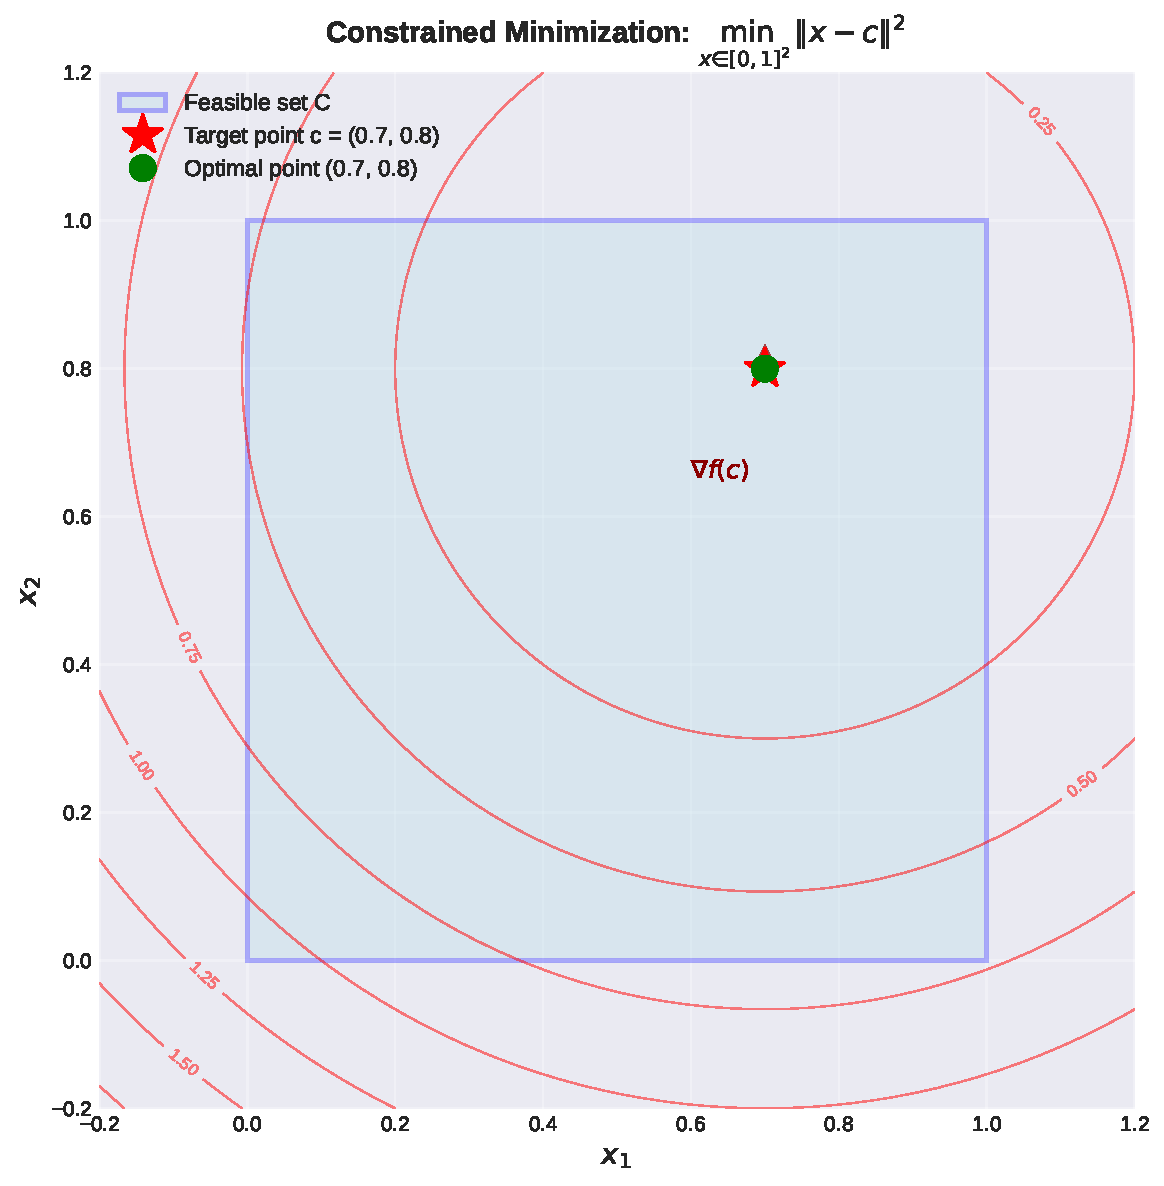
\includegraphics[width=\textwidth]{fig_constrained_opt.pdf}

The optimizer is the projection of $c$ onto the feasible set $[0,1]^2$.

\end{frame}

% Section 27.3
\section{27.3 Affine Constraints}

\begin{frame}[allowframebreaks]
\frametitle{Affine Constraints: Lagrange Multipliers}

\textbf{Problem with Affine Constraints:}

Consider the problem:
\[\min_{x \in H} f(x) \quad \text{subject to} \quad Lx = r\]

where $f \in \Gamma_0(H)$, $L \in \mathcal{B}(H, K)$, and $r \in L(\text{dom } f)$.

\vspace{0.3cm}

\textbf{Proposition 27.14:} $\bar{x}$ is a solution if and only if:
\[L\bar{x} = r \quad \text{and} \quad (\exists \bar{v} \in K)\ -L^*\bar{v} \in \partial f(\bar{x})\]

In this case, $\bar{v}$ is a \textbf{Lagrange multiplier}.

\vspace{0.3cm}

\textbf{When $f$ is Gâteaux differentiable:}
\[L\bar{x} = r \quad \text{and} \quad (\exists \bar{v} \in K)\ \nabla f(\bar{x}) = -L^*\bar{v}\]

\vspace{0.3cm}

\textbf{Key Insight:}
The solution satisfies both the constraint and a subdifferential condition involving Lagrange multipliers.

\end{frame}

\begin{frame}[fragile]
\frametitle{Affine Constraints: Python Example}

\begin{lstlisting}[language=Python]
import numpy as np
from scipy.optimize import minimize

# Minimize ||x||^2 subject to x_1 + x_2 + x_3 = 1
# Exact solution: x = (1/3, 1/3, 1/3)

def f(x):
    return np.sum(x**2)

def grad_f(x):
    return 2 * x

# Affine constraint: Ax = b
A = np.array([[1, 1, 1]])
b = np.array([1.0])

def constraint(x):
    return A @ x - b

x0 = np.array([0.0, 0.0, 0.0])

# Solve with constraint
from scipy.optimize import LinearConstraint
lc = LinearConstraint(A, b, b)
result = minimize(f, x0, jac=grad_f, constraints=lc)

x_opt = result.x
print(f"Optimal solution: {x_opt}")
print(f"Constraint check: {A @ x_opt}")
print(f"Optimal value: {f(x_opt):.6f}")

# Theoretical: x* = (1/3, 1/3, 1/3)
x_theo = np.ones(3) / 3
print(f"Theoretical: {x_theo}")
print(f"Match: {np.allclose(x_opt, x_theo, atol=1e-5)}")
\end{lstlisting}

\end{frame}

\begin{frame}[allowframebreaks]
\frametitle{Special Cases of Affine Constraints}

\textbf{Case 1: Finite-Dimensional Non-negativity Constraints}

Let $A \in \mathbb{R}^{M \times N}$, $f \in \Gamma_0(\mathbb{R}^N)$. Consider:
\[\min_{x \in \mathbb{R}_+^N} f(x) \quad \text{subject to} \quad Ax \in \mathbb{R}_+^M\]

The KKT conditions characterize solutions.

\vspace{0.3cm}

\textbf{Case 2: Linear Programming Constraints}

For polyhedral sets $C$ and $D$ with $C \cap L^{-1}(D) \neq \varnothing$:
\[\min_{x \in C} f(x) + g(Lx)\]
where $f = \iota_C$ and $g = \iota_D$.

The solution satisfies normal cone conditions.

\vspace{0.3cm}

\textbf{Corollary 27.15 (Closed Convex Sets):}

For closed convex sets $C$ and $D$ with $f = \iota_C$, $g = \iota_D$:
\[x \in \mathbb{R}^M \text{ and } (\exists u \in K^\perp \cap \partial f(\bar{x}))\ \langle \bar{x} - y \mid u \rangle \leq 0 \quad (\forall y \in C)\]

\end{frame}

% New Section: More General Results
\section{27.4 Further Applications}

\begin{frame}[allowframebreaks]
\frametitle{Composite Functions: Corollary 27.3}

\textbf{Corollary 27.3:} Let $f, g \in \Gamma_0(H)$, $\bar{x} \in H$, and $\gamma \in \mathbb{R}_{++}$.

Suppose one of these conditions holds:
\begin{enumerate}
    \item[(a)] $0 \in \text{sri}(\text{dom } g - \text{dom } f)$
    \item[(b)] $H$ finite-dimensional, $g$ polyhedral, $\text{dom } g \cap \text{ri}(\text{dom } f) \neq \varnothing$
    \item[(c)] $H$ finite-dimensional, $f, g$ polyhedral, $\text{dom } f \cap \text{dom } g \neq \varnothing$
\end{enumerate}

\textbf{Then these are equivalent:}
\begin{enumerate}
    \item[(i)] $\bar{x}$ is a solution to $\min_x f(x) + g(x)$
    \item[(ii)] $\bar{x} \in \text{zer}(\partial f + \partial g)$
    \item[(iii)] $\bar{x} \in \text{Prox}_g(\text{Fix}(2\text{Prox}_f - \text{Id}) \circ (2\text{Prox}_g - \text{Id}))$
    \item[(iv)] $(\exists u \in \partial g(\bar{x}))\ -u \in \partial f(\bar{x})$
    \item[(v)] $(\exists u \in \partial f(\bar{x}))\ -u \in \partial g(\bar{x})$
    \item[(vi)] $(\exists u \in \partial g(\bar{x}))(\forall y \in H)$ $\langle \bar{x} - y \mid u \rangle + f(\bar{x}) \leq f(y)$
\end{enumerate}

When $g$ is Gâteaux differentiable at $\bar{x}$:
\begin{itemize}
    \item $-\nabla g(\bar{x}) \in \partial f(\bar{x})$
    \item $(\forall y \in H)$ $\langle \bar{x} - y \mid \nabla g(\bar{x}) \rangle + f(\bar{x}) \leq f(y)$
    \item $\bar{x} = \text{Prox}_{\gamma f}(\bar{x} - \gamma \nabla g(\bar{x}))$
\end{itemize}

\end{frame}

\begin{frame}[fragile]
\frametitle{Composite Optimization: Python Example}

\begin{lstlisting}[language=Python]
import numpy as np
from scipy.optimize import minimize
from scipy.sparse.linalg import cg

# Minimize ||x - x0||^2 + lambda * ||x||_1
# (quadratic + sparsity-inducing term)
# Solution: soft thresholding

x0 = np.array([1.5, 0.3, -2.0, 0.1, 0.8])
lam = 0.5

def f(x):
    return np.sum((x - x0)**2)

def f_sparse(x):
    return np.sum((x - x0)**2) + lam * np.sum(np.abs(x))

# Solve
result = minimize(f_sparse, x0, method='L-BFGS-B')
x_opt = result.x

# Soft thresholding: x* = sign(x0) * max(|x0| - lam/2, 0)
x_analytical = np.sign(x0) * np.maximum(np.abs(x0) - lam/2, 0)

print(f"Numerical solution:  {x_opt}")
print(f"Analytical (soft-thresh): {x_analytical}")
print(f"Match: {np.allclose(x_opt, x_analytical, atol=1e-4)}")
\end{lstlisting}

\end{frame}

% Examples Section
\section{27.5 Detailed Examples}

\begin{frame}[allowframebreaks]
\frametitle{Example 27.10: Projection onto a Convex Set}

\textbf{Problem:} Project a point $p$ onto a closed convex set $C$.

\[\min_{x \in C} \|x - p\|^2\]

\vspace{0.2cm}

\textbf{Solution:} The projection $\bar{x} = P_C(p)$ is characterized by:
\[\langle p - \bar{x} \mid y - \bar{x} \rangle \leq 0 \quad \forall y \in C\]

This means $(p - \bar{x})$ is orthogonal to $C$ at $\bar{x}$.

\vspace{0.3cm}

\textbf{Verification with Fermat's Rule:}
\begin{itemize}
    \item Objective: $f(x) = \frac{1}{2}\|x - p\|^2$
    \item Gradient: $\nabla f(x) = x - p$
    \item Normal cone to $C$ at $\bar{x}$: $N_C(\bar{x})$
    \item Condition: $-\nabla f(\bar{x}) = p - \bar{x} \in N_C(\bar{x})$ (correct)
\end{itemize}

\end{frame}

\begin{frame}[fragile]
\frametitle{Example 27.10: Python Visualization}

\begin{lstlisting}[language=Python]
import numpy as np
import matplotlib.pyplot as plt
from scipy.spatial import ConvexHull

# Define a convex polygon
vertices = np.array([[0, 0], [2, 0], [2.5, 1.5],
                     [1, 2], [0, 1.5]])
hull = ConvexHull(vertices)

# Point to project
p = np.array([1.5, -0.5])

# Simple projection by checking distance to vertices
# and edges (numerical approach)
from scipy.optimize import minimize

def dist_sq(x):
    return np.sum((x - p)**2)

# Start from a point in the hull
x0 = np.mean(vertices, axis=0)

# Constraint: point in convex hull
# Use linear constraints from convex hull equations
A_ub, b_ub = [], []
for simplex in hull.simplices:
    # For each edge/facet, create inequality constraint
    pass

result = minimize(dist_sq, x0, method='Nelder-Mead')
x_opt = result.x

print(f"Point to project: {p}")
print(f"Projection: {x_opt}")
print(f"Distance: {np.sqrt(dist_sq(x_opt)):.4f}")
\end{lstlisting}

\end{frame}

\begin{frame}[allowframebreaks]
\frametitle{Example 27.11 and 27.12: Bilinear Forms}

\textbf{Example 27.11 (Stampacchia):} Let $F : H \times H \to \mathbb{R}$ be bilinear with:
\[(\forall x, y \in H)\ |F(x, y)| \leq \beta\|x\|\|y\| \quad \text{and} \quad F(x, x) \geq \alpha\|x\|^2\]

For a nonempty closed convex set $C$ and $\ell \in \mathcal{B}(H, \mathbb{R})$:
\[\exists! \bar{x} \in C : (\forall y \in C)\ F(\bar{x}, y - \bar{x}) \geq \ell(y - \bar{x})\]

\textbf{Applications:}
\begin{itemize}
    \item Variational inequalities
    \item Nonlinear elasticity problems
    \item Convex optimization with indefinite quadratic objectives
\end{itemize}

\vspace{0.3cm}

\textbf{Example 27.12 (Lax-Milgram):} Similar structure but for optimization:
\[\min_{x \in C} \left\{\frac{1}{2}F(x, x) - \ell(x)\right\}\]

The unique minimizer satisfies the variational inequality.

\end{frame}

% Summary and Key Takeaways
\section{Summary}

\begin{frame}[allowframebreaks]
\frametitle{Key Theorems and Results}

\textbf{Main Contributions:}

\begin{enumerate}
    \item \textbf{Fermat's Rule:} $x^* \in \text{Argmin}(f) \iff 0 \in \partial f(x^*)$

    \item \textbf{Composite Minimization:} Conditions for minimizing $f(x) + g(Lx)$

    \item \textbf{Constrained Minimization:} Characterizations using normal cones

    \item \textbf{Affine Constraints:} Lagrange multiplier conditions

    \item \textbf{Variational Inequalities:} Connection to monotone operators

    \item \textbf{Regularity Conditions:} Sufficient conditions for equivalences
\end{enumerate}

\vspace{0.3cm}

\textbf{Practical Implications:}
\begin{itemize}
    \item First-order optimality conditions for nonsmooth convex optimization
    \item Foundation for proximal algorithms
    \item Characterization of solutions without explicit computation
    \item Extension to infinite-dimensional settings
\end{itemize}

\end{frame}

\begin{frame}
\frametitle{Connections to Other Chapters}

\begin{itemize}
    \item \textbf{Subdifferentials} (Ch. 16): Necessary tools for stating conditions

    \item \textbf{Monotone Operators} (Ch. 20): $\partial f$ is maximally monotone

    \item \textbf{Resolvents} (Ch. 23): Connection to proximal point algorithm

    \item \textbf{Projection Operators} (Ch. 24): Special case of minimization

    \item \textbf{Splitting Methods} (Ch. 22): Algorithms based on Fermat's rule

    \item \textbf{Proximal Algorithms} (Ch. 28): Direct application to minimization
\end{itemize}

\end{frame}

\end{document}
